%
% $RCSfile: chain_of_responsibility.tex,v $
%
% Copyright (C) 2002-2008. Christian Heller.
%
% Permission is granted to copy, distribute and/or modify this document
% under the terms of the GNU Free Documentation License, Version 1.1 or
% any later version published by the Free Software Foundation; with no
% Invariant Sections, with no Front-Cover Texts and with no Back-Cover
% Texts. A copy of the license is included in the section entitled
% "GNU Free Documentation License".
%
% http://www.cybop.net
% - Cybernetics Oriented Programming -
%
% http://www.resmedicinae.org
% - Information in Medicine -
%
% Version: $Revision: 1.1 $ $Date: 2008-08-19 20:41:05 $ $Author: christian $
% Authors: Christian Heller <christian.heller@tuxtax.de>
%

\subsubsection{Chain of Responsibility}
\label{chain_of_responsibility_heading}
\index{Chain of Responsibility Pattern}
\index{Composite Pattern}
\index{Recursion}
\index{Event Handler Pattern}
\index{Bureaucrat Pattern}
\index{Responder Pattern}
\index{Hierarchical Model View Controller Pattern}
\index{HMVC}
\index{Bidirectional Dependency}
\index{Strong Coupling between Layers}

The \emph{Chain of Responsibility} pattern \cite{gamma1995} is similar to the
\emph{Composite}, in that it represents a recursive structure as well. Objects
destined to solve a task are linked with a corresponding \emph{Successor}
(figure \ref{chain_figure}), such forming a chain. If an object is not able to
solve a task, that task is forwarded to the object's successor, along the chain.

\begin{figure}[ht]
    \begin{center}
        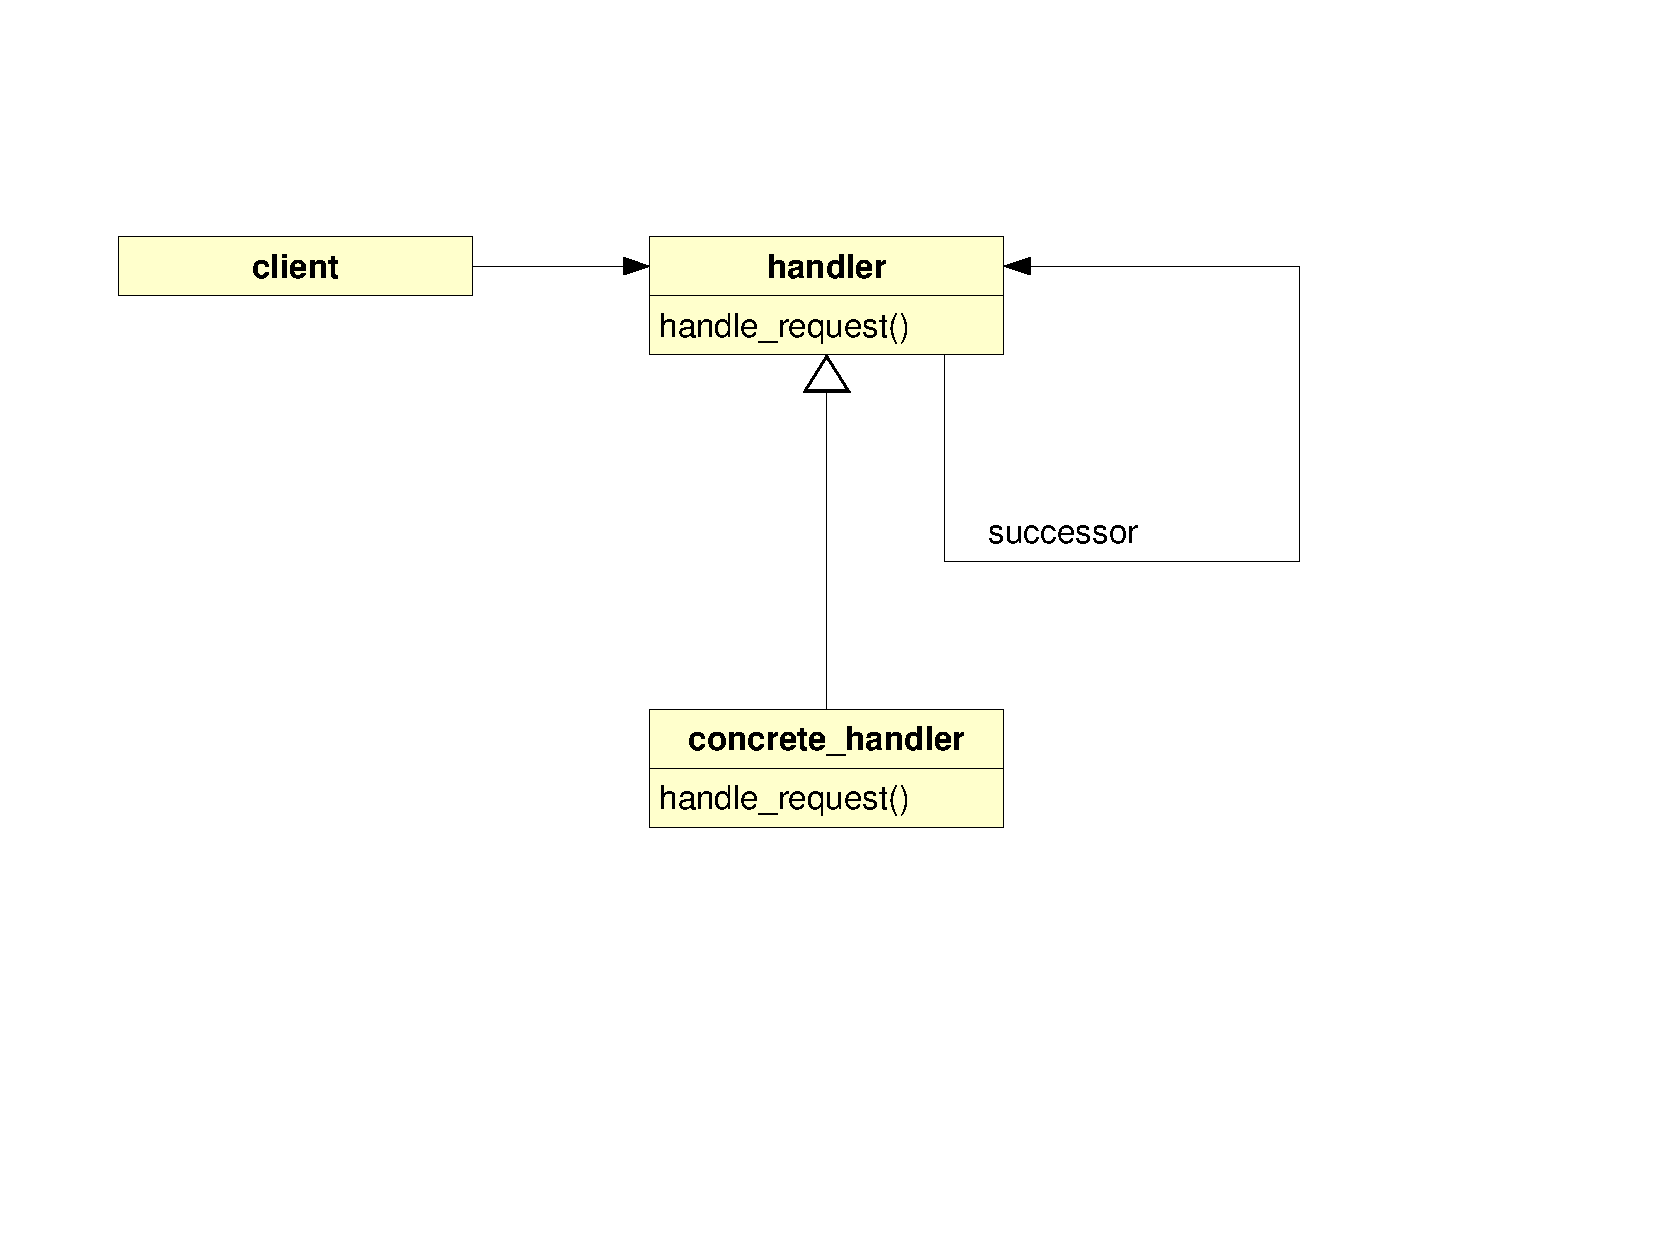
\includegraphics[scale=0.3,angle=-90]{graphic/chain.pdf}
        \caption{Chain of Responsibility Pattern}
        \label{chain_figure}
    \end{center}
\end{figure}

The pattern found wide application, for example in help systems, in event
handling frameworks or for exception handling. Its \emph{Handler} class is
known under synonyms like \emph{Event Handler}, \emph{Bureaucrat} or
\emph{Responder}. Frequently, the pattern gets misused by delegating messages
not only to children but also to the parent of objects. The
\emph{Hierarhical Model View Controller} (HMVC) pattern (section
\ref{hierarchical_model_view_controller_heading}) is one example for this. It
causes unfavourable bidirectional dependencies and leads to stronger coupling
between the layers of a framework, because parent- and child objects then
reference each other.

Much like state knowledge (data structures) is representable by the knowledge
schema being described in chapter \ref{knowledge_schema_heading}, also logic
knowledge (algorithms, operations) is. A compound logic model may contain
further logic models, which it calls or sends as signal in a manner similar to
the \emph{Chain of Responsibility} principle.
